\documentclass{standalone}
\usepackage[usenames,dvipsnames,svgnames,table]{xcolor}
\usepackage{tikz}
\usetikzlibrary{arrows.meta}
\tikzset{>={Latex[width=5mm,length=5mm]}}

\title{Evilness versus IQ}

\begin{document}
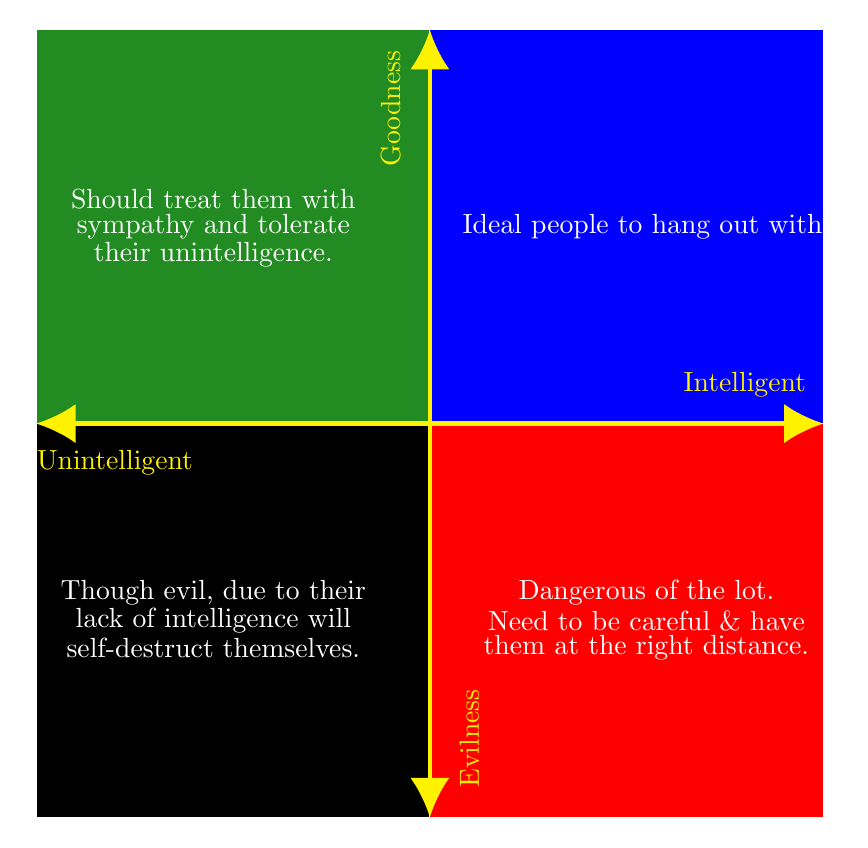
\begin{tikzpicture}
%First quadrant
\draw [draw=white,fill=blue] (0,0) rectangle (5,5);
\node at (2.75,2.5) {\color{white}Ideal people to hang out with.};

%Second quadrant
\draw [draw=white,fill=ForestGreen] (0,0) rectangle (-5,5);
\node at (-2.75,2.85) {\color{white}Should treat them with};
\node at (-2.75,2.5) {\color{white}sympathy and tolerate};
\node at (-2.75,2.15) {\color{white}their unintelligence.};

%Third quadrant
\draw [draw=white,fill=black] (0,0) rectangle (-5,-5);
\node at (-2.75,-2.15) {\color{white}Though evil, due to their};
\node at (-2.75,-2.5) {\color{white}lack of intelligence will};
\node at (-2.75,-2.85) {\color{white}self-destruct themselves.};

%Fourth quadrant
\draw [draw=white,fill=red] (0,0) rectangle (5,-5);
\node at (2.75,-2.15) {\color{white}Dangerous of the lot.};
\node at (2.75,-2.5) {\color{white}Need to be careful \& have};
\node at (2.75,-2.85) {\color{white}them at the right distance.};

\draw [draw=yellow, ultra thick, <->] (-5,0) -- (5,0);
\draw [draw=yellow, ultra thick, <->] (0,-5) -- (0,5);
\node [rotate=90] at (0.5,-4) {\color{yellow}Evilness};
\node [rotate=90] at (-0.5,4) {\color{yellow}Goodness};
\node [rotate=0] at (4,0.5) {\color{yellow}Intelligent};
\node [rotate=0] at (-4,-0.5) {\color{yellow}Unintelligent};


\end{tikzpicture}

\end{document}